\documentclass{article}

\usepackage[utf8]{inputenc}
\usepackage[T1]{fontenc}
\usepackage{geometry}
\usepackage{xcolor}
\usepackage{graphicx}
\usepackage{subcaption}
\usepackage{verbatim}
\usepackage{amsmath,amssymb}
\usepackage{amstext}
\usepackage{amsthm}
\usepackage{steinmetz}
\usepackage{stackrel}
\usepackage{mathtools}
\geometry{a4paper}

\usepackage[english]{babel}
\frenchspacing

\counterwithin{figure}{section}
\counterwithin{table}{section}

\title{Ale's report}
\author{Alessandro Matteo Rossi}
\date{data}

\begin{document}
\maketitle




\tableofcontents

\clearpage
\section{Processing}

After the two numbers have been inserted by the user they reach the processing section of the circuit. In this phase the numbers get summed or subtracted, depending on the user's choice. In figure \ref{Processing_Total} the processing section of the circuit, highlighted in green.

\begin{figure}[h]
  \centering
  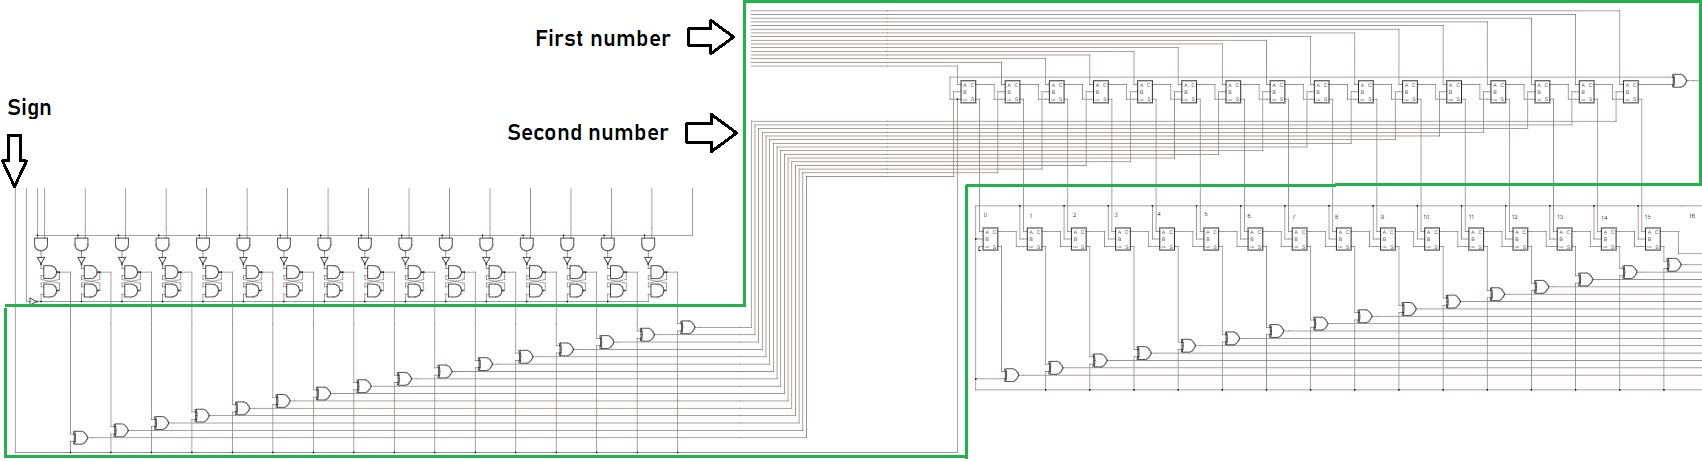
\includegraphics[scale=0.43]{SC_Processing_Total.JPG}
  \caption{Picture the circuit processing part (highlighted in green)}
  \label{Processing_Total}
\end{figure}

The processing is split in two subphases:
\begin{itemize}
  \item During the first subphase the second number, memorized in the flip-flop memory (left side of figure \ref{Processing_Total}) gets inverted if the user picked the subtraction operation, otherwise it does not get modified.
  \item The algebrical sum happens in the top right side of the circuit.
\end{itemize}

Regarding the first point, the first mandatory step is to invert the number. We remember that the opposite of a binary number $A$ is
\begin{equation}
-A=NOT(A)+1
\label{Law}
\end{equation}
and we also remember that in the Boolean Algebra factors can commute during a sum.

So, first of all, we perform the NOT operation in figure \ref{Processing1} thanks to XOR gates. They compare the sign of the second number with the bits, one at a time, and if the sign is negative (the sign line in figure \ref{Processing1}, highlighted in red) they invert the bit. Otherwise nothing happens.

\begin{figure}[h]
  \centering
  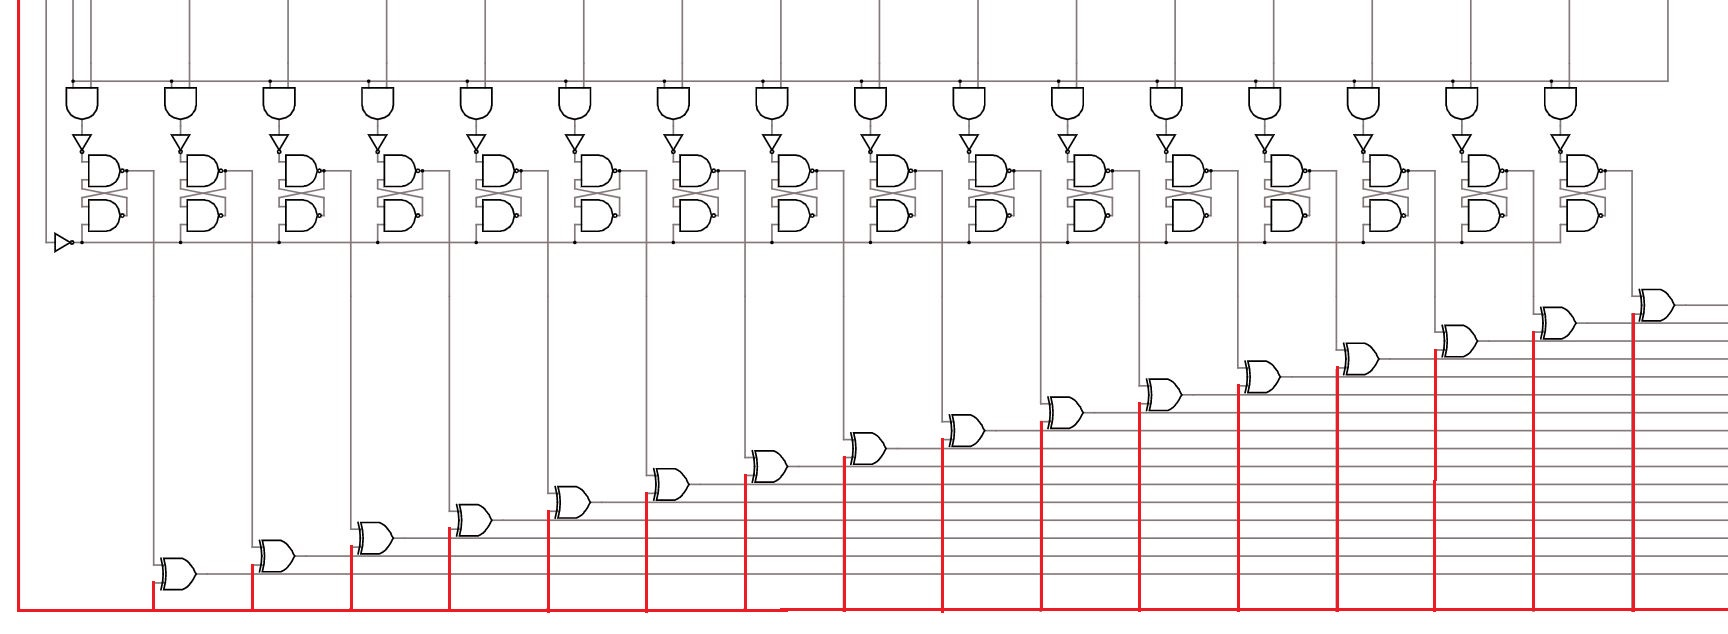
\includegraphics[scale=0.35]{SC_Processing1.JPG}
  \caption{Picture of the inverting part, with the sign wire highlighted in red}
  \label{Processing1}
\end{figure}

Regarding the second point, this is not only where a unit gets added to the second number (equation \ref{Law}) but also where the algebrical sum between the two inputs happens.

This sum is performed by a \textit{ripple carry adder} (shown in figure \ref{RCA} in green), which is composed by a series of full adders, highlighted in blue. The sign wire keeps being red.

\begin{figure}[h]
  \centering
  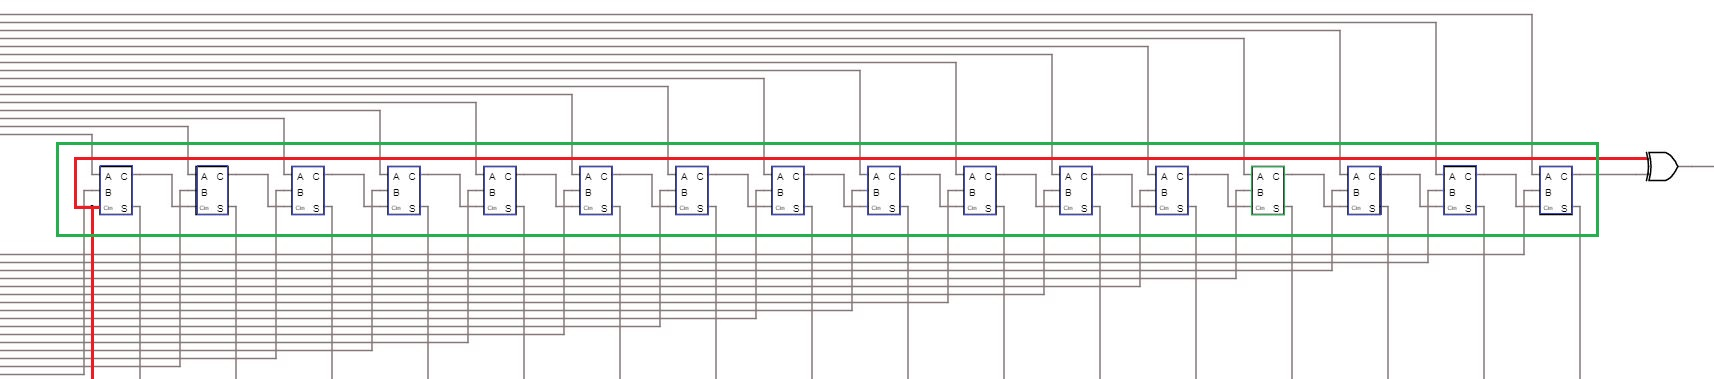
\includegraphics[scale=0.43]{SC_Processing2.JPG}
  \caption{Picture of the ripple carry adder part, with the sign wire highlighted in red and the full adders highlighted in blue}
  \label{RCA}
\end{figure}

The ripple carry adder (shortened in RCA) is an $B$-bit adder circuit composed of $B$ full adders. 

A single full adder is a 3 input bits adder, with a 2-bit output. Its inputs are a number $A$, a number $B$ and a carry-over produced in a previous operation, whereas the outputs are a result $S$ and a carry-over $C_{out}$. Its table of truth is figure \ref{FullAdder}, where the input carry-over is $C_{in}$ and the output one is $C_{out}$.

\begin{table}[h]
  \centering
  \begin{tabular}{|| c | c | c || c | c ||}
  \hline
  A$_1$ & A$_2$ & C$_{in}$ & S & C$_{out}$ \\ \hline
  0 & 0 & 0 & 0 & 0 \\ \hline
  0 & 1 & 0 & 1 & 0 \\ \hline
  1 & 0 & 0 & 1 & 0 \\ \hline
  1 & 1 & 0 & 0 & 1 \\ \hline
  0 & 0 & 1 & 1 & 0 \\ \hline
  0 & 1 & 1 & 0 & 1 \\ \hline
  1 & 0 & 1 & 0 & 1 \\ \hline
  1 & 1 & 1 & 1 & 1 \\ \hline
  \end{tabular}
  \label{FullAdder}
\end{table}

By aligning $B$ full adders is possible to sum (or subtract) two $B$-bit numbers. Considering that, as already mentioned, if the number is negative it is needed to invert the number and sum 1, the ripple carry adder allows the circuit to:
\begin{itemize}
  \item Sum two numbers if they are both positive, with no action performed from the inverting part of the processing circuit.
  \item Subtract one number from another by inverting the second number, as already explained, and summing 1 as the first $C_{in}$ of the first full adder of the RCA.
\end{itemize}
  
In conclusion, the output moves to the decoding part of the circuit, that will allow the circuit to show the result on displays. Moreover, a XOR gate checks the relation among the sign bit and the carry-over of the last full adder. This happens because the sign of the final result depends on the relation among the modules of the two numbers, and if the first one is bigger than the other, the result will be surely positive, otherwise negative.





\clearpage
\section{Decoder}

After the inputs have been processed (added or subtracted), it is needed a decoder (see figure \ref{Decoder}) in order to convert the output from binary number to its decimal form. Considering that this 16-bit calculator allows the user to insert numbers within the range (INSERIRE IL RANGE CAZZO), the operative boundary of this calculator is (INSERIRE).

\vspace{3mm}

The largest number that can be shown as result is around $\pm$INSERIER (+INSERIER or -INSERIER, to be exact), both positive and negative. So the decoding circuit needs to have 6 led displays for the digits and one extra display for the sign.

\vspace{3mm}

We decided to operate the binary-decimal conversion with the so called "double dabble" circuit, that will be explained later in the report. Nevertheless this was not the main problem. The double-dabble converts positive numbers perfectly, but not negative ones. The major issue was to adapt this circuit to work with both positive and negative numbers. 

The representation of the negative binary numbers follows the "two's complement" rule. It means that taken a B number of bits, all the numbers that can be represented with a 0 in the $B-1$ position are considered positive, otherwise they are negative. This allows to split the 17 bits available in two sets of 16 bits, and so it is possible to have the range described above.

\begin{figure}[h]
    \centering
    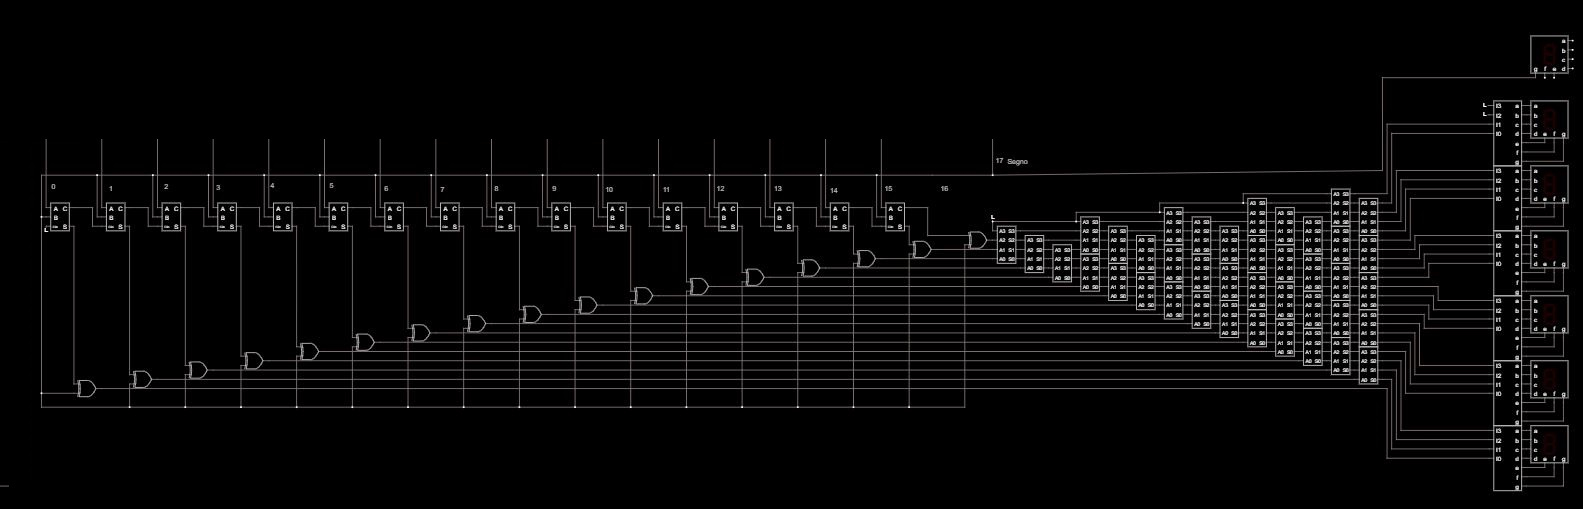
\includegraphics[scale=0.43]{SC_Decoder.JPG}
    \caption{Picture of the decoder}
    \label{Decoder}
  \end{figure}

\subsection{About the number sign}

The number sign has to be taken into account before converting the number into its decimal form. The number is a 16-bit binary, as already said, and it has one extra bit for the sign, the 16th bit.


This part of the circuit (represented in figure \ref{Converter}) uses full-adders and XOR logic gates, components that got already discussed in the previous sections. After the processing of the operation between the two inputs, the first 16 bits reach the A input of a specific full adder (the green lines in figure \ref{Converter}), whereas the sign bit follows the red path.

This 16th bit reaches every B input of all the full adders, and also the XOR gates, that compare the result of the single full adders with the 16th bit. The sign bit is true (or 1) when the number is negative and 0 otherwise. This allows the full adders to sum 1, following the formula above, if the processing output is negative, whereas if it is positive the number just stays the same.

After this, the XOR gates, which table of truth is 
\begin{center}
\begin{tabular}{||c|c||c||}
    \hline
    A & B & A XOR B \\
    \hline
    0 & 0 & 0 \\
    \hline
    0 & 1 & 1 \\
    \hline
    1 & 0 & 1 \\
    \hline
    1 & 1 & 0 \\
    \hline
\end{tabular}
\end{center}

give the final result, which will go to the double dabble. Considering the full adder output as "A" for the XOR, and the sign bit as "B", it is possible to deduct that when the sign is false (so the processing output is positive) the XOR gates do not modify the full adder output (which do not work too, considering that their "B", the sign bit, is false as well). When the XOR "B" is true (so the processing output is negative), the XOR gives the opposite of its "A" as output.

\begin{figure}[h]
    \centering
    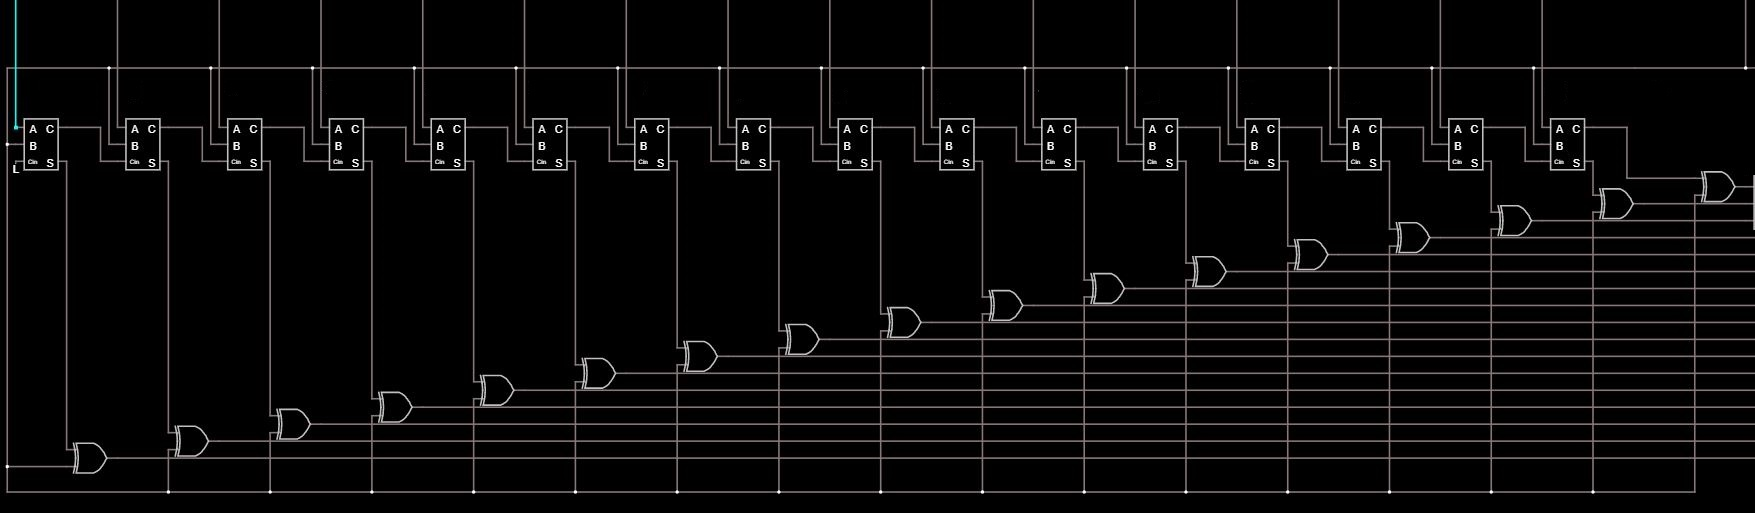
\includegraphics[scale=0.43]{SC_Converter.JPG}
    \caption{Picture of the first part of the decoder}
    \label{Converter}
  \end{figure}

\subsection{Double dabble}

This second part of the decoder is reached by the number that needs to be converted into decimal form. 

The entire circuit relies on an algorithmic process based on the concept of "shift and add 3", which is the name of the component that mostly populates figure \ref{DoubleDabble}.

This algorithm takes a binary number and after having processed it gives an output divided into smaller parts composed of 4 bits each. Everyone of these parts will be then elaborated by 7 segment decoders and represent a single digit of the decimal number. The 7-segment decoders are obviously connected to 7-segments led displays, that can be seen on the right side of figure \ref{DoubleDabble}.

\begin{figure}[h]
    \centering
    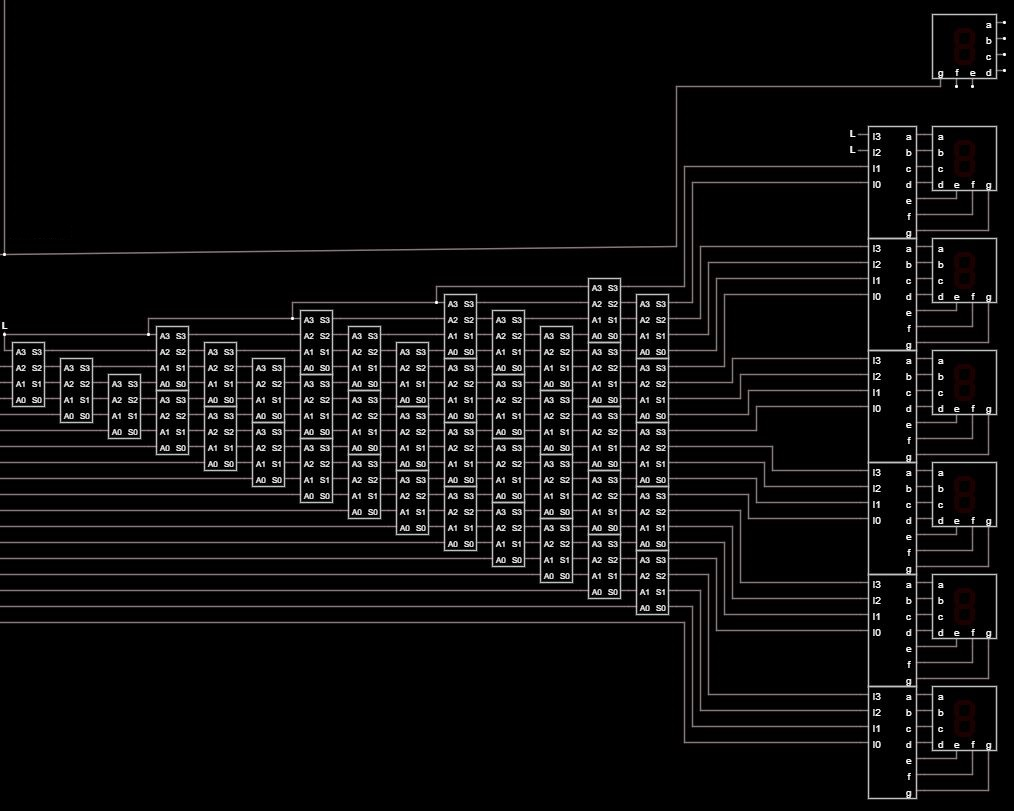
\includegraphics[scale=0.43]{SC_DoubleDabble.JPG}
    \caption{Picture of the double dabble, the second part of the circuit}
    \label{DoubleDabble}
  \end{figure}


The algorithm works as follows (graphic representation in figure \ref{SC_Algo}):
\begin{enumerate}
  \item Let's consider a 8-bit binary number, but the same argument works for n bits. 
  \item Let's consider the units, as long as that binary value is lower or equal to 4, the binary input can keep shifting and increasing the units.
  \item When the units value is an integer greater than 4, 3 is added to them and the shifting process continues.
\end{enumerate}

It is mandatory to add 3 because during the conversion the weight of the 4 bits of the unit is 16, at maximum, whereas those for digits represent a maximum of 10 in decimal form. So to compensate this loss, we add a half of the lost weight.

\begin{table}[h]
  \centering
  \begin{tabular}{||c|c|c|c||c||c||}
    \hline
    \# & Hundreds & Tens & Units & Binary & Operation \\
    \hline
    1 & 0000 & 0000 & 0000 & 11111111 & Start \\
    2 & 0000 & 0000 & 0001 & 11111110 & Shift1 (every 4-bit slot < 5) \\
    3 & 0000 & 0000 & 0011 & 11111100 & Shift2 (every 4-bit slot < 5) \\ 
    4 & 0000 & 0000 & 0111 & 11111000 & Shift3 (every 4-bit slot < 5) \\
    5 & 0000 & 0000 & 1010 & 11110000 & Add-3 to "Units" ("Units" $\geq$ 5)\\
    6 & 0000 & 0001 & 0101 & 11110000 & Shift4 (every 4-bit slot < 5) \\
    7 & 0000 & 0001 & 1000 & 11110000 & Add-3 to "Units" ("Units" $\geq$ 5)\\
    8 & 0000 & 0011 & 0001 & 11100000 & Shift5 (every 4-bit slot < 5) \\
    9 & 0000 & 0110 & 0011 & 11000000 & Shift6 (every 4-bit slot < 5) \\
    10 & 0000 & 1001 & 0011& 11000000 & Add-3 to "Tens" ("Tens" $\geq$ 5)\\
    11 & 0001 & 0010 & 0111& 10000000 & Shift7 (every 4-bit slot < 5) \\
    12 & 0001 & 0010 & 1010& 10000000 & Add-3 to "Units" ("Units" $\geq$ 5)\\
    13 & 0010 & 0101 & 0101& 00000000 & Shift8 (every 4-bit slot < 5) \\
    \hline
  \end{tabular}
    \label{SC_Algo}
    \caption{Double dabble algorithm applied to the decimal number 255}

  \end{table}


The goal of the "Shift and add 3" component, programmed using the customizable logic of the simulator, is to operate this shift or addition depending on the 4 inputs given. Its table of truth is figure \ref{Add3Table}.

\begin{table}[h]
  \centering
  \begin{tabular}{||c|c||}
    \hline
    Input & Output \\
    \hline
    0000 & 0000 \\
    0001 & 0001 \\
    0010 & 0010 \\ 
    0011 & 0011 \\
    0100 & 0100 \\
    0101 & 1000 \\
    0110 & 1001 \\
    0111 & 1010 \\
    1000 & 1011 \\
    1001 & 1100 \\
    \hline
  \end{tabular}
    \label{Add3Table}
    \caption{"Shift and add 3" table of truth}
  \end{table}

It is clear, thanks to this figure, that when the number is greater than four it gets added three to it. The "shift" part can be seen in figure \ref{DoubleDabble}. If we consider the input A0 of a single Add3 component, when can see that its output, S0, is the input A1 for the next component.

After all this process the number is divided into 4 bit groups that enter the 7-segment decoders and than display the result.








\end{document}